\section{Описание использованного алгоритма}

% 1
\begin{figure}[H]
  \centering
  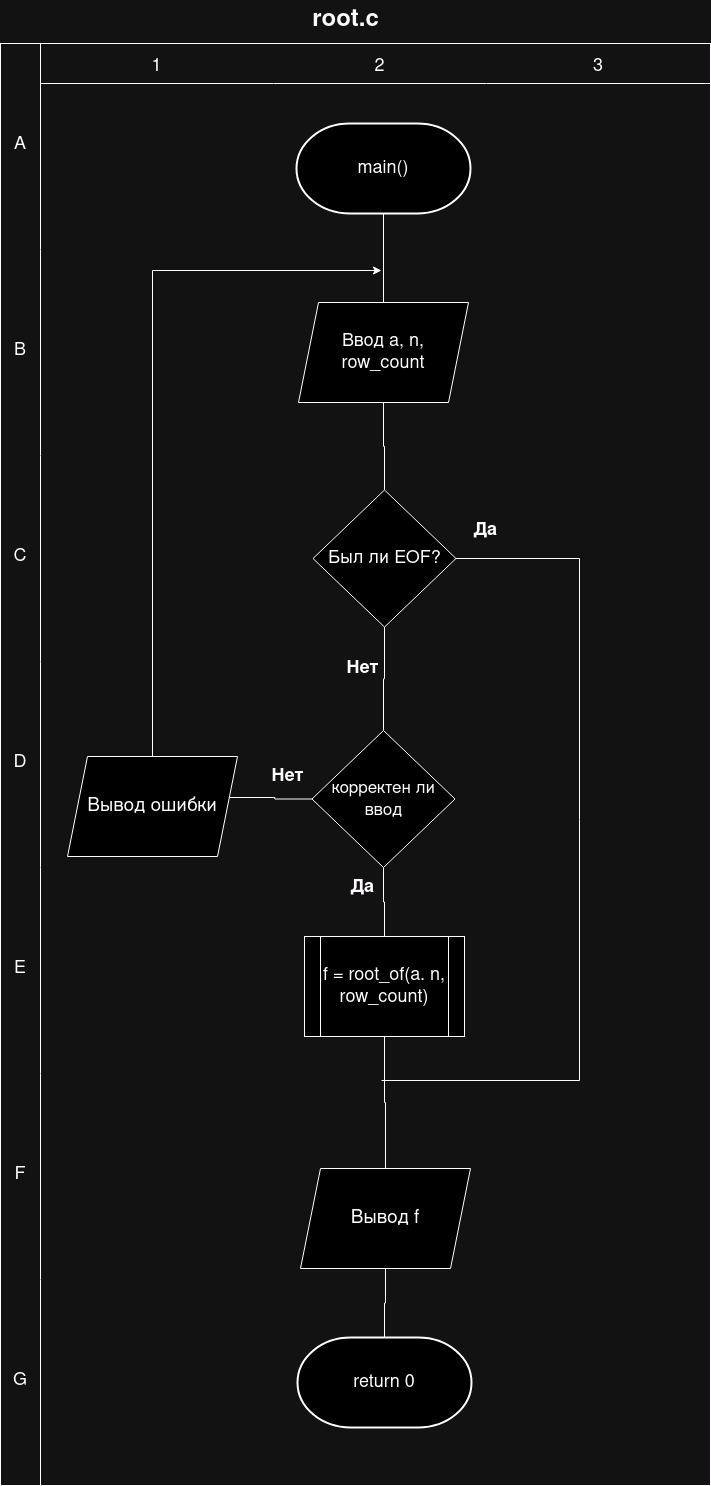
\includegraphics[width=0.65\textwidth,height=0.9\textheight,keepaspectratio]{block_schemes/1_root_function_main}
  \caption{Блок-схема алгоритма работы функции \texttt{main()} для программы \texttt{root}}
\end{figure}

% 2
\begin{figure}[H]
  \centering
  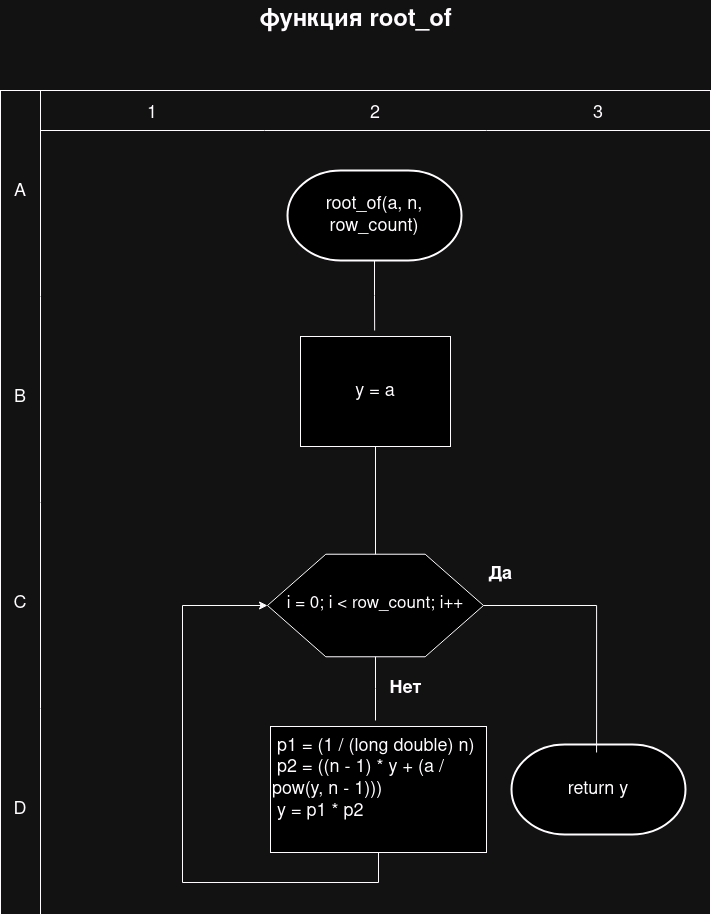
\includegraphics[width=0.7\textwidth]{block_schemes/3_root_function_root_of}
  \caption{Блок-схема алгоритма работы функции \texttt{root\_of()} для программы \texttt{root}}
\end{figure}

% 3
\begin{figure}[H]
  \centering
  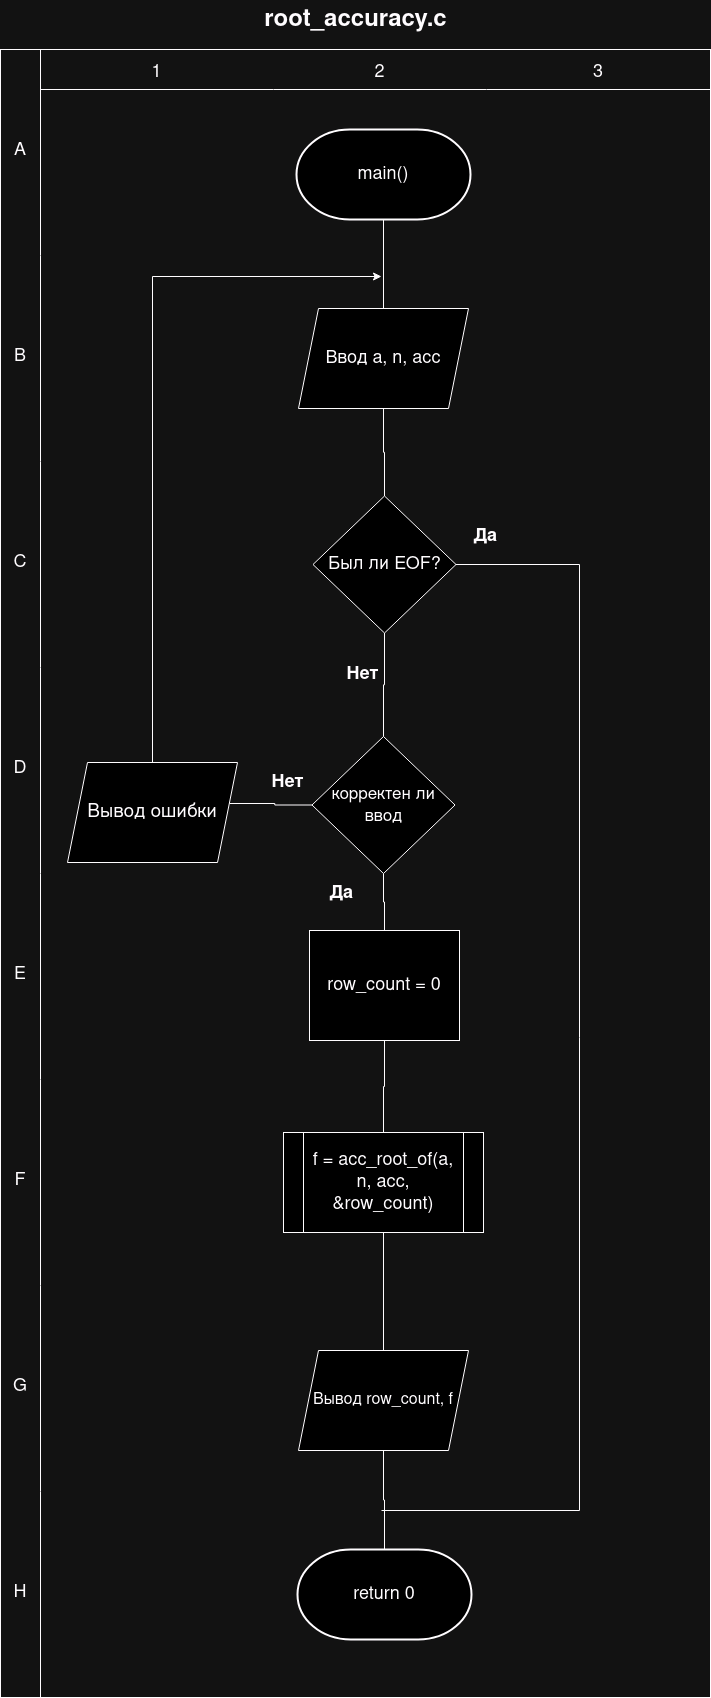
\includegraphics[width=\textwidth,height=\textheight,keepaspectratio]{block_schemes/5_root_accuracy_function_main}
  \caption{Блок-схема алгоритма работы функции \texttt{main()} для программы \texttt{root\_accuracy}}
\end{figure}

% 4
\begin{figure}[H]
  \centering
  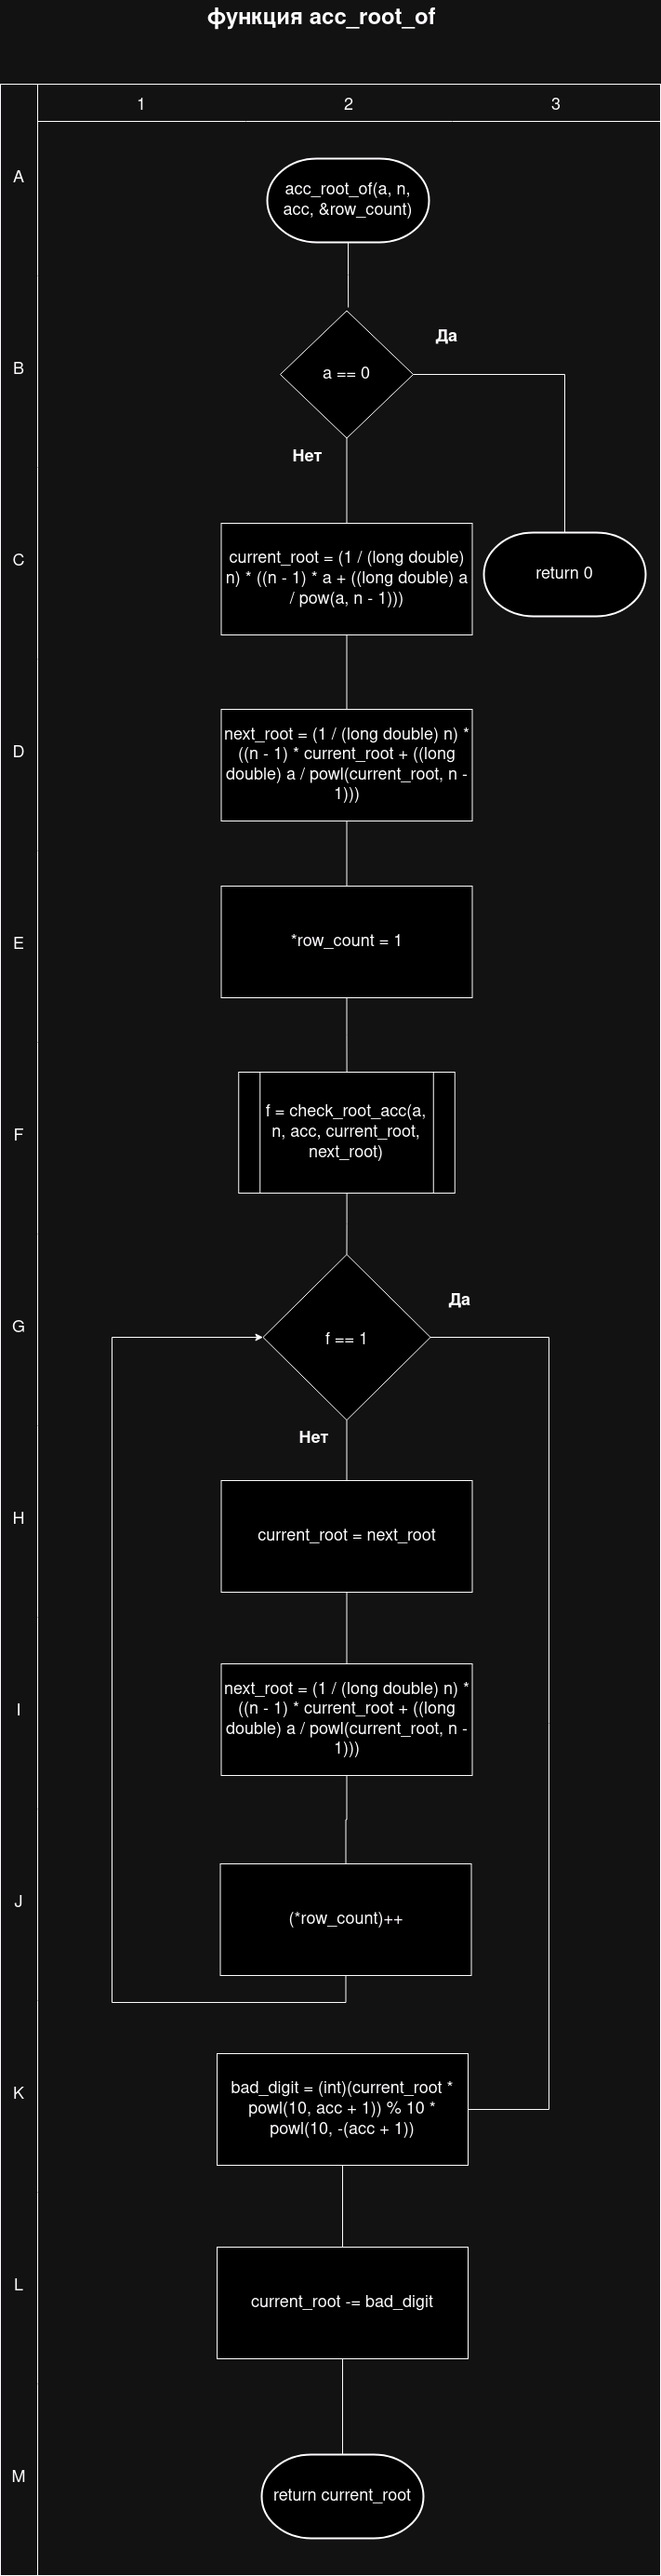
\includegraphics[trim={0 1450 0 0}, clip, width=0.7\textwidth]{block_schemes/7_root_accuracy_function_acc_root_of}
  \phantomcaption
\end{figure}

\begin{figure}[H]
\ContinuedFloat
  \centering
  % 711x2769 pixels
  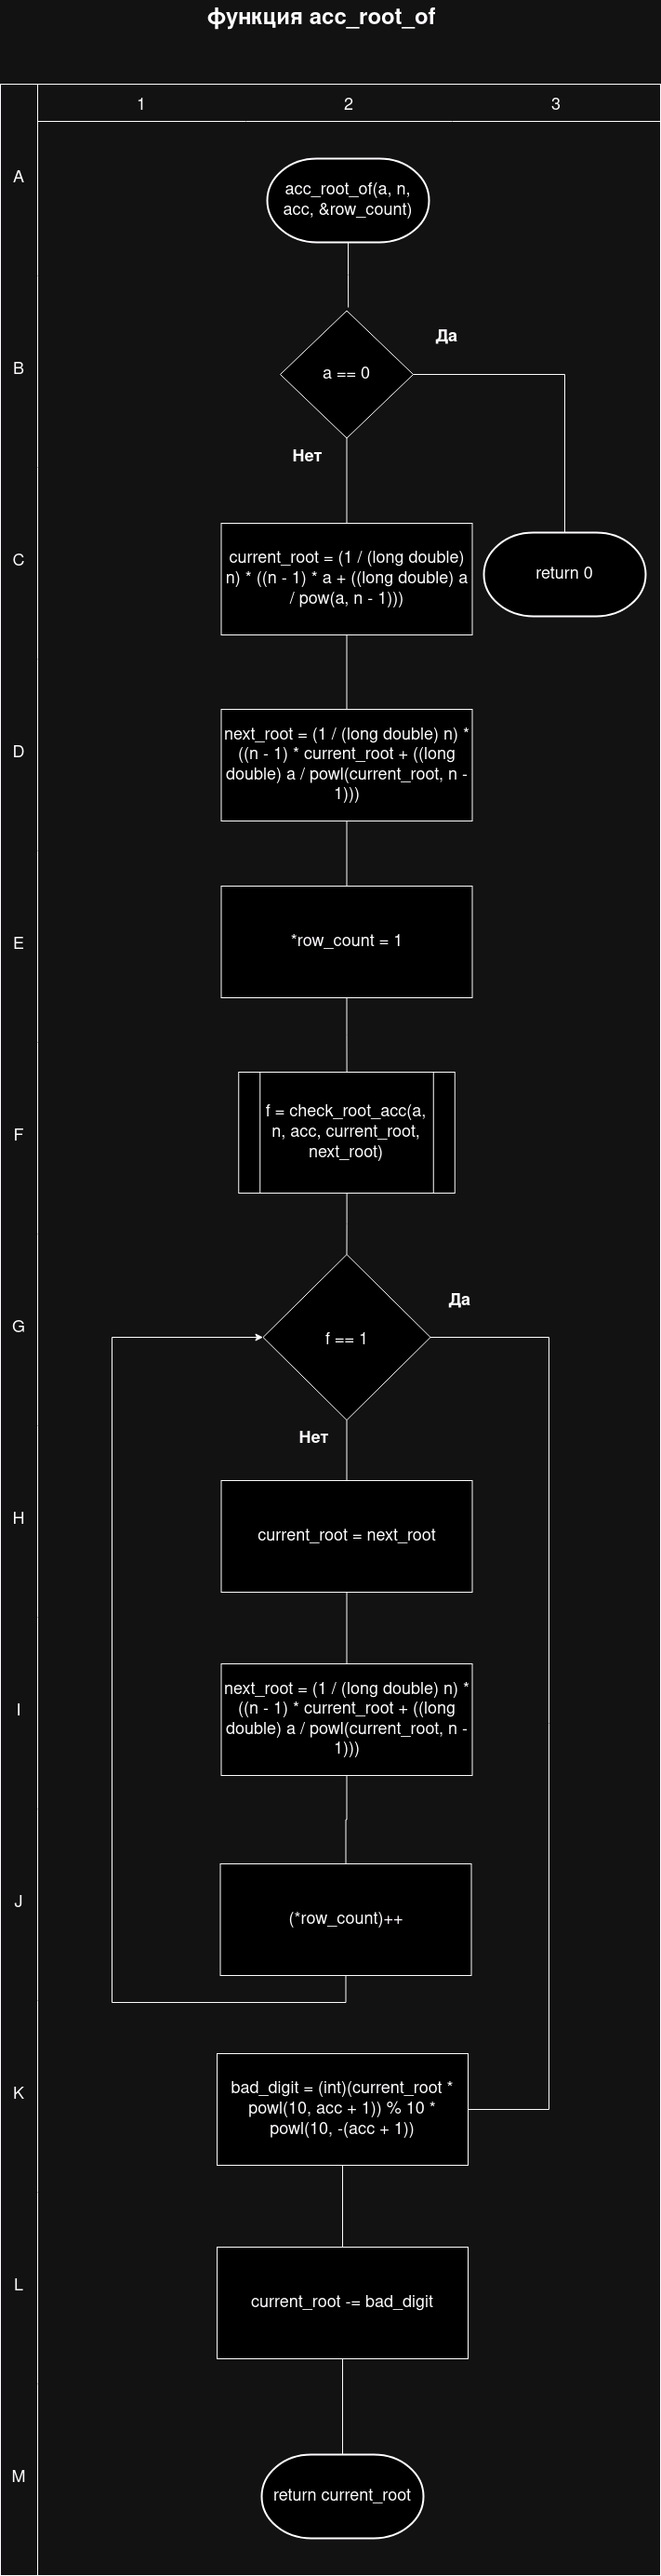
\includegraphics[trim={0 0 0 1300}, clip, width=0.7\textwidth, height=\textheight]{block_schemes/7_root_accuracy_function_acc_root_of}
  \caption{Блок-схема алгоритма работы функции \texttt{acc\_root\_of()} для программы \texttt{root\_accuracy}}
\end{figure}

% 5
\begin{figure}[H]
  \centering
  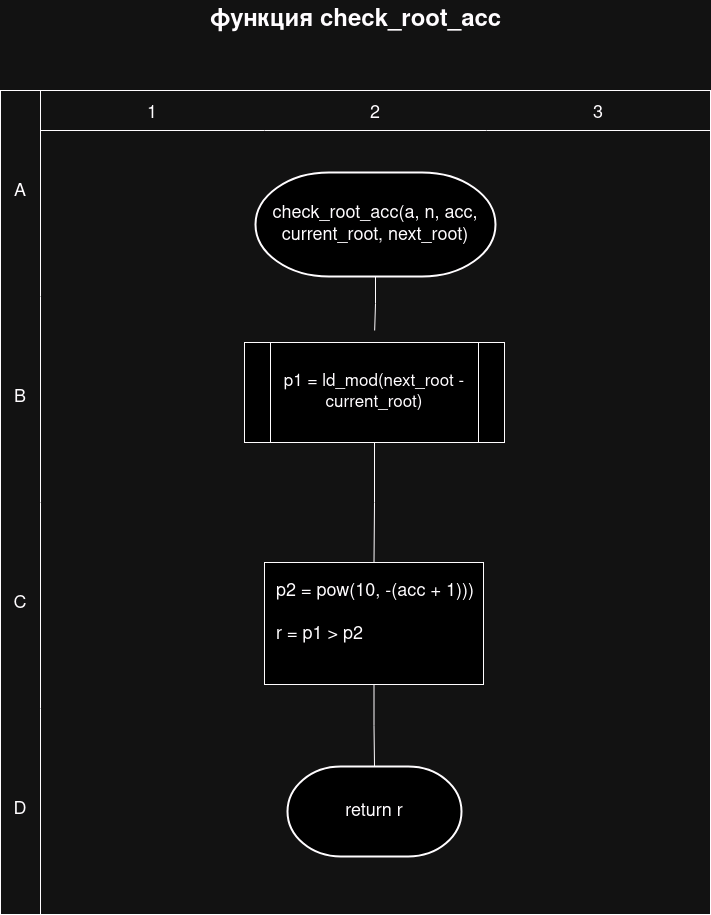
\includegraphics[width=0.9\textwidth,height=0.8\textheight,keepaspectratio]{block_schemes/9_root_accuracy_function_check_root_acc}
  \caption{Блок-схема алгоритма работы функции \texttt{check\_root\_acc()} для программы \texttt{root\_accuracy}}
\end{figure}

% 6
\begin{figure}[H]
  \centering
  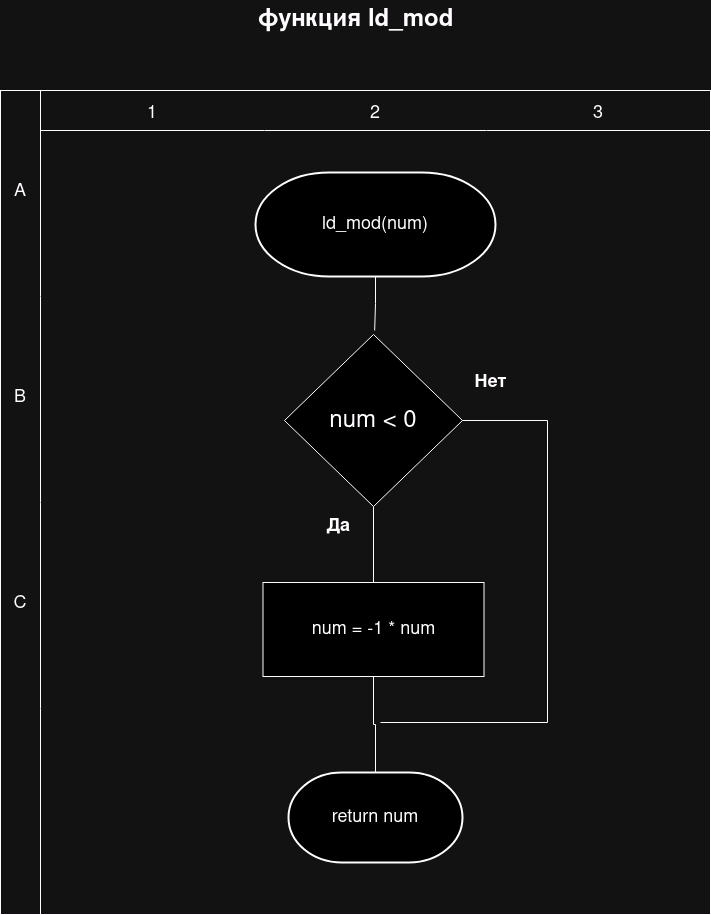
\includegraphics[width=0.9\textwidth,height=0.8\textheight,keepaspectratio]{block_schemes/11_root_accuracy_function_ld_mod.png}
  \caption{Блок-схема алгоритма работы функции \texttt{ld\_mod()} для программы \texttt{root\_accuracy}}
\end{figure}
